\section{Hardware}
\label{hardware}
%todo:clean this up
One of the main goals of this research was to give the designer flexibility in choosing the appropriate sensors for a given flight test. To this end, hardware that is available in breakout boards was given preference, since it gives the aircraft designer more flexibility. The aircraft designer could utilize surface mount components if vehicle integration space is extremely limited, or can use the available breakout boards to make circuit-level integration easier if vehicle space is not a driving flight test concern.
\subsection*{Flight Computer}
The flight computer chosen was an Arduino Due. This board has a 32-bit ARM processor, 54 digital I/O pins, 12 analog input pins, and 2 analog output pins. The main driver in the decision to use an Arduino-based platform was the vast support community, which allows quicker code development. The Arduino also offers a package that integrates well into most of the available airframes, and the stackable header pins allowed for easy integration with other boards. The Due in particular was chosen as it is (at the time of writing) the most advanced Arduino available. The main advantages it has over the comparable Arduino Mega is its increased clock speed (84 MHz for the Due\cite{Atmel2012} vs 16 MHz for the Arduino Mega\cite{Atmel2012atmega}) and its 32-bit architecture (vs. 8-bit for the Arduino Mega).
\nomenclature{I/O}{Input-output}
\begin{figure}[H]

  \centering
    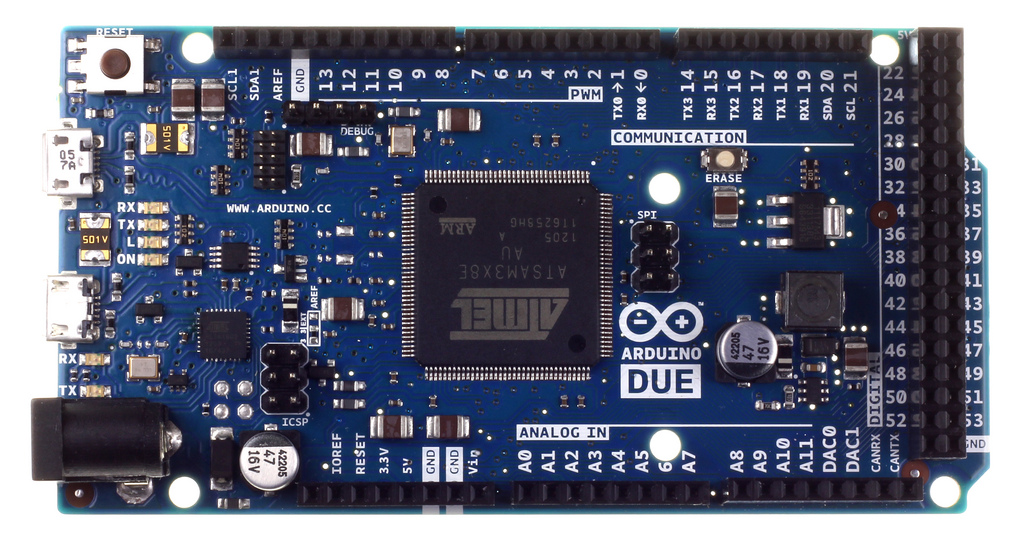
\includegraphics[width=0.3\textwidth]{figures/arduinoDue.jpg}\  \caption{Arduino Due Flight Computer} \label{arduinoPicture}
\end{figure}

The Arduino Due uses a 3.3V architecture instead of the usual Arduino architecture, which uses a 5V operating voltage. This was mainly beneficial, since most of the selected sensors used 3.3V as both supply and logic voltage. Logic level circuits, shown in Figure \ref{logicLevel}, were used to translate to 5V signals where required.  The board is powered through the 3.5mm barrel jack, using a 3-cell LiPo battery, with a nominal voltage of 11.1V.
\nomenclature{LiPo}{Lithium polymer}
\begin{figure}[H]

  \centering
    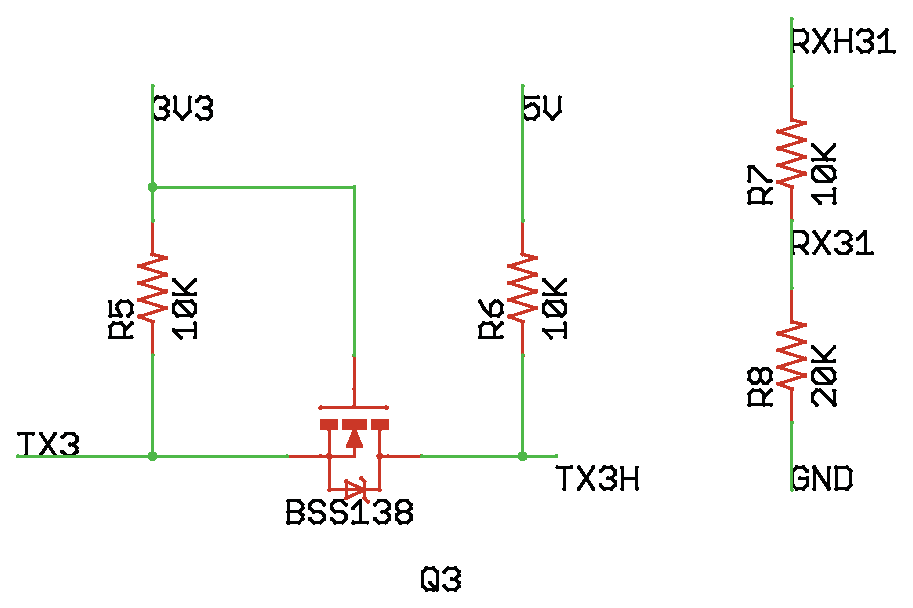
\includegraphics[width=0.3\textwidth]{figures/logicLevelConverterSchematic.eps}
      \caption{Logic Level Converter Circuit} \label{logicLevel}
\end{figure}

\subsection*{Accelerometer}
The accelerometer chosen for the data acquisiton system was the ADXL-362 from Analog Devices. It has a noise error of $175\mu\text{G}/\sqrt{\text{Hz}}$ and uses a 3.3V digital SPI interface\cite{adxl362DataSheet}. The accelerometer is in an LGA package and was surface mounted to the main PCB.
\nomenclature{SPI}{Serial peripheral interface}
\nomenclature{LGA}{Land grid array}
\nomenclature{G}{Gravity}
\nomenclature{PCB}{Printed circuit board}
\begin{figure}[H]

  \centering
    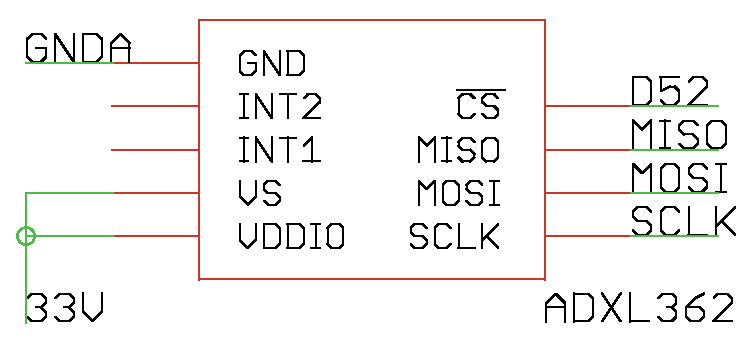
\includegraphics[width=0.3\textwidth]{figures/adxl362.eps}
      \caption{ADXL-362 Schematic} \label{adxl362Schematic}
\end{figure}

The accelerometer is calibrated in the field through an optimization routine using MATLAB's \texttt{fmincon} nonlinear constrained optimization function. For any given orientation, the accelerometer's reading can be expressed as
\begin{align}
\label{accelCalibFit}
\begin{bmatrix}
r_x & 0 & 0\\ 0 & r_y & 0\\ 0 & 0 & r_z
\end{bmatrix} 
\begin{bmatrix}
m_x \\ m_y \\ m_z
\end{bmatrix} 
+ \begin{bmatrix}
b_x & b_y & b_z
\end{bmatrix}&= \begin{bmatrix} (G_x-a_x) & (G_y - a_y) & (G_z - a_z) \end{bmatrix}
\end{align}
\noindent
where the $r$ terms are the bit readings from the accelerometer for each axis, the $m$ terms are the slope of a linear fit for each axis, the $b$ terms are the zero offset of a linear fit for each axis, and the $a$ terms are the actual accelerations.
 
 The slope and offset terms can be found through field calibration and a nonlinear optimization routine. The algorithm uses the fact that, while in a static orientation, the magnitude of the measured vector should be exactly 1G. The optimization problem is then

\begin{align}
\underset{x}{\text{minimize }} f(x) &= \sqrt{(1G-|(\vec{t})|)^2}
\end{align}
\noindent
where $\vec{t}$ is the right hand side of Equation \ref{accelCalibFit}, and the variable of interest $x$ is the vector of slopes and offsets in Equation \ref{accelCalibFit}. The slope terms in $x$ are constrained to be positive. To be a deterministic system of equations, at least six static orientations are required. To avoid the noise of a single reading, the problem was expanded to take 100 data points in six different static orientations, and Equation \ref{accelCalibFit} was expanded to become a least squares problem. The main benefit of this technique is that field calibration can be accomplished without needing precise knowledge of the orientation of gravity with respect to the sensor during the calibration routine. When tested, the results of the calibration were consistent between this algorithm and using known orientations. For error propagation, the noise during calibration was taken as the sensor's noise level.
%todo:include accelerometer calibration plots sent to McDonald. also, make plot of linear fits and the RMS noise to show noise levels. Histograms?

\subsection*{Vehicle Mass}
All test vehicles were weighed using a U-Line H-1650 counting scale. The scale has an accuracy of 0.001 lbs and a maximum capacity of 30 lbs. The minimum capacity of the scale is 10 grams \cite{U-Line}.
\subsection*{Magnetometers}
Two separate magnetometers were used for separate purposes. A Honeywell HMR-2300 3-D magnetometer, shown in Figure \ref{hmr23000Picture}, is the main magnetometer. It is used when extremely accurate heading information is needed, or when GPS course is unavailable, such as during extremely slow or vertical flight.

\begin{figure}[H]

  \centering
    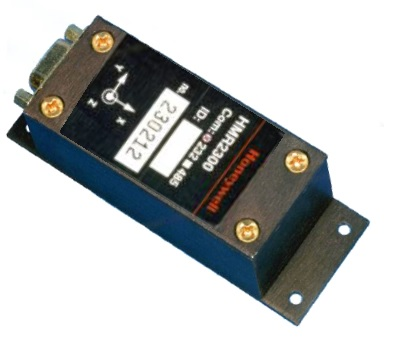
\includegraphics[width=0.3\textwidth]{figures/hmr2300.jpg}
      \caption{Honeywell HMR-2300 3-D Magnetometer } \label{hmr23000Picture}
\end{figure}

%todo:take gauss to angles
This magnetometer provides a RMS error of 0.1 milliGauss for all axes, using the 1 Gauss full-scale setting\cite{hmr2300DataSheet}.
\nomenclature{RMS}{Root mean squared}
The HMR-2300 can be supplied with power between 6V and 15V, so the 3-cell 11.1V nominal LiPo battery that powers the Arduino also passes through to power the magnetometer. The HMR-2300 operates using an RS-232 serial interface. To properly interface with the Arduino Due, which uses 3.3V TTL logic levels, a Max-3232 IC was used. This IC, when combined with charge pump capacitors, translates TTL levels between 3V and 5.5V to RS-232 logic levels of $\pm6$V.
\nomenclature{IC}{Integrated circuit}
%todo:update this schematic, and include a picture of board layout?
 \begin{figure}[H]

   \centering
     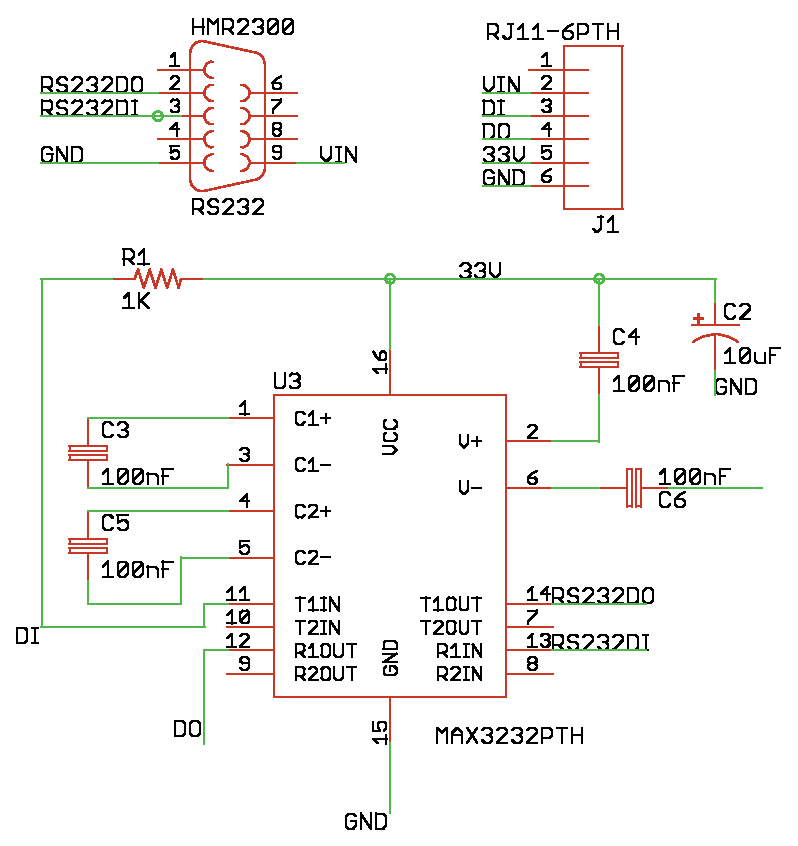
\includegraphics[width=0.7\textwidth]{figures/magBoard.eps}
        \caption{HMR-2300 Logic Level Circuit} \label{magBoardSchematic}
 \end{figure}
 
 The second magnetometer is a Honeywell HMC-5883L, which comes in an LCC package that was surface mounted to the main sensor board. It was added to the system for two main reasons: it is much smaller for applications where size is critical, and it is much less expensive for testing with unproven vehicles. It communicates with the Arduino using an I$^2$C interface and uses a 3.3V operating voltage\cite{hmc5883LDatasheet}. The HMC-5883L has an accuracy of 2 milliGauss on each axis. \nomenclature{LCC}{Leadless chip carrier}
 
 \begin{figure}[H]

   \centering
     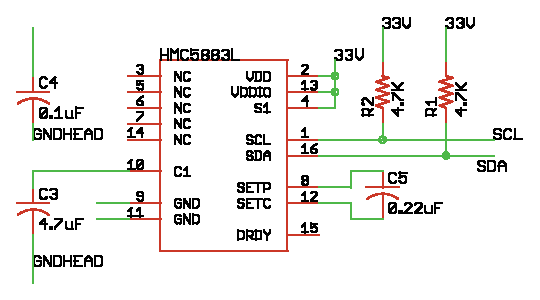
\includegraphics[width=0.5\textwidth]{figures/hmc5883LSchematic.eps}
        \caption{HMC-5883L Schematic} \label{hmc5883LSchematic}
 \end{figure}

 Both magnetometers were calibrated for both soft-iron and hard-iron effects\cite{magCalibration}. To do this, data was acquired for 10 seconds with the magnetometer being swept through all directions. An ellipsoid was fit to the data using a ordinary least squares method available from the MATLAB file exchange\cite{ellipsoidFit}.
 The least squares fit estimates the center and radius of each axis. The center values for each axis was subtracted from the readings to remove hard-iron effects. Each $i$-th axis is then scaled by $\frac{1}{R_i}$ to reshape the ellipse into a circle, which removes soft-iron effects.
 
 The surface-mounted HMC-5883L was assumed to be aligned with the surface-mounted accelerometer. Since the two magnetometers both measured the North vector, a rotation matrix that describes the difference in alignment between the two sensors can be calculated by
 \begin{align}
\vec{N}_{HMC5883} &= \bar{R}^{M_1}_b\vec{N}_{HMR2300}.
 \end{align}
 
 The rotation matrix $\bar{R}^{M_1}_b$ can then be used to align the HMR-2300's coordinate system with the body mounted accelerometers, using
 \begin{align}
\vec{N}_b &= \bar{R}^{M_1}_b\vec{N}_{HMR2300}.
 \end{align}
 
\subsection*{Gyroscope}
A three-axis gyroscope was also included in the system. The gyroscope chosen was the Invensense ITG-3200, which comes in a QFN package.\nomenclature{QFN}{Quad-flats no-leads} This gyroscope has a total error of $0.38^\circ/$s-rms\cite{itg3200DataSheet}, and uses a digital I$^2$C interface on a 3.3V operating voltage. This gyroscope has a full-scale span of $\pm2000^\circ/$s.
\nomenclature{I$^2$C}{Inter-integrated circuit}

\begin{figure}[H]

  \centering
    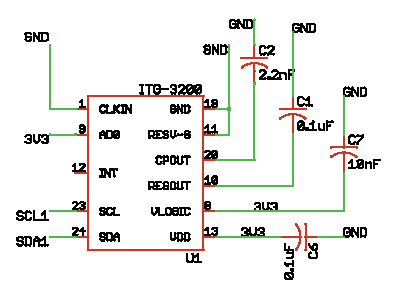
\includegraphics[width=0.5\textwidth]{figures/itg3200Schematic.eps}
      \caption{ITG-3200 Eagle Schematic} \label{itg3200Schematic}
\end{figure}

The gyroscope was calibrated in the same manner as the accelerometer. The device was placed in six orientations on a turn table which rotated at a constant 33 $\frac{1}{3}$ RPM. Slope and offset values for each axis were calculated using \texttt{fmincon}. Before each flight test, the offset values were re-calculated by taking 10 seconds of static readings.\\
\nomenclature{RPM}{Rotations per minute}

\subsection*{Air Data System}
A five-hole probe was chosen to measure aerodynamic angles as they do not contain moving parts and can provide very accurate, repeatable data. The five-hole probe selected was the Aeroprobe Air Data probe. It is 6 inches long, has a diameter of 1/8 inch, and uses a 0.25" hexagonal section as it's mounting section. The probe comes factory calibrated from angles to pressure readings, and was calibrated at an airspeed of 70 ft/s.\\
%todo:document calibration process
The probe was extended roughly one chord length in front of the leading edge of the wing by a 0.25" carbon fiber tube and an aluminum adapter which connected to the probe using set screws.
\begin{figure}[H]

  \centering
    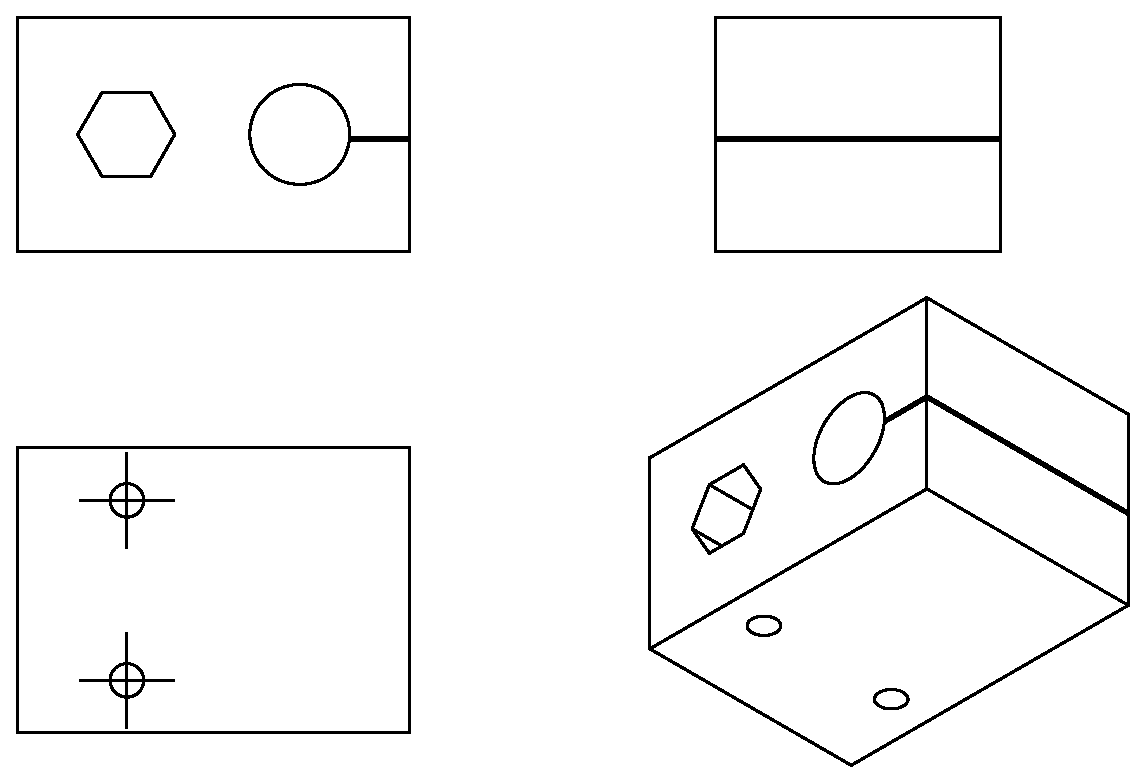
\includegraphics[width=.5\textwidth]{figures/probeAdapter.eps}
      \caption{Five-Hole Probe Adapter} \label{fig:probeAdapter}
\end{figure}
The adapter was manufactured to be square to itself and to have the reference flat of the probe's hexagonal section be parallel to one side of the adapter. An accelerometer was then glued to a side of the adapter, and the accelerometer was calibrated to the block using a level surface and the flat sides of the adapter. Before each flight test, three static readings are taken of the adapter's accelerometer and the main body-mounted accelerometer. Since the probe's orientation with respect to the adapter's accelerometer is known, this allows the wind angles measured by the probe to be calculated with respect to the body axes, and gives an accurate alignment of the wind reference frame to the body reference frame.\\

 Each pair of lines of the five-hole air data probe is connected to an All Sensors digital differential pressure sensor with a full scale range of $\pm$5 in-H$_2$O\cite{allsensorsDDO}. The static port of the five-hole probe was connected to an All Sensors BARO-DO digital barometric pressure sensor,which has a range of 600 to 1100 mBar\cite{allSensorsBaroDatasheet}. The barometric pressure sensor comes in the same package and uses the same communication protocol as the differential pressure sensors.

\begin{figure}[H]

  \centering
    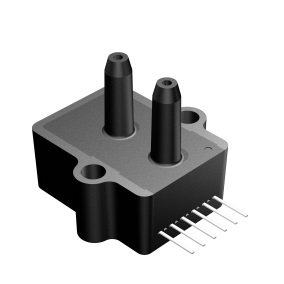
\includegraphics[width=0.25\textwidth]{figures/allsensorsPressure.jpg}
      \caption{All Sensors 5-INCH-D-DO Pressure Sensor} \label{allsensorsPressurePic}
\end{figure}

The differential pressure sensors have a total error band of 0.25\% FSO, and the barometric pressure sensor has a nominal error of 1 mBar. They use a UART serial interface that operates on a 5V logic level, so the logic levels were converted to the 3.3V levels of the Arduino Due. The serial interface includes addressable read commands, which allows multiple devices on a single bus, and ensures all devices record pressure at the same time. The sensor can output both a 14-bit pressure reading and a 12-bit temperature reading, which the device uses to correct its pressure measurement.\\

A digital temperature sensor was combined with the barometric pressure sensor to estimate the air density, which allowed air speed to be calculated.

\begin{figure}[H]

  \centering
    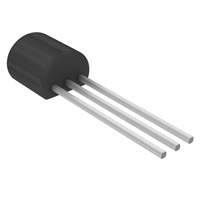
\includegraphics[width=0.15\textwidth]{figures/ds18b20Picture.jpg}
  \caption{Dallas Semiconductors' DS18B20 Digital Temperature Sensors} \label{ds18b20Picture}
\end{figure}
 The DS18B20 from Dallas Semiconductors was chosen for its relatively simple One-Wire interface. The device can be powered with the communication line and has a $\pm$0.5$^\circ$C nominal accuracy\cite{DS18B20Datasheet}.

The differential pressure sensors were calibrated for slope using a Reference Pressure Recorder from Crystal Engineering\cite{pressCalib}. This calibration unit is capable of 0.025\% of reading. The zero offset of each differential pressure sensor was removed before each flight by taking 100 data samples in a no-wind condition. The barometric pressure transducer and the temperature sensor were calibrated for offset using a Paroscientific Model 745 Pressure Standard, capable of $0.008\%$ FSO accuracy\cite{pressureStandard}. \nomenclature{FSO}{Full scale output}

\subsubsection*{Wind Angle Kalman Filter}

To improve the accuracy of the wind angle estimation, a discrete Extended Kalman filter was used. The state transition functions are
\begin{align}
\dot{\alpha} & = \frac{1}{V\cos\beta}(-a_x\sin\alpha+a_z\cos\alpha)+q-(p\cos\alpha+r\sin\alpha)\tan\beta\\
\dot{\beta} &=\frac{1}{V}(-a_x\cos\alpha\sin\beta+a_y\cos\beta-a_z\sin\alpha\sin\beta)+p\sin\alpha-r\cos\alpha.
\end{align}

These state transition equations come from solving for the vehicle forces in wind axes instead of body axes\cite{klein2006aircraft}. The equations for the Kalman filter for the wind angles are
\begin{align}
\begin{bmatrix}
\alpha_k\\\beta_k
\end{bmatrix} &= \begin{bmatrix}
1& 0\\0&1
\end{bmatrix}\begin{bmatrix}
\alpha_{k-1}\\\beta_{k-1}
\end{bmatrix}+\begin{bmatrix}
\Delta T& 0\\0&\Delta T
\end{bmatrix}\begin{bmatrix}
\dot{\alpha_{k}}\\\dot{\beta_{k}}
\end{bmatrix}+\hat{w}_{k-1}\\
z_k & = \begin{bmatrix}
1 & 0\\0&1
\end{bmatrix}\begin{bmatrix}
\alpha_{k}\\
\beta_{k}
\end{bmatrix}+\hat{v}_{k-1}.
\end{align}

The process covariance matrix was calculated using the error propagation discussed in Section \ref{pointErrorSection} and the standard deviation data from the zero offset calibration of each of the applicable sensors. The measurement noise covariance matrix was calculated based on the standard deviation data for the zero offset of each pressure transducer connected to the five-hole probe.

\subsection*{GPS Receiver}
A uBlox LEA-6T GPS receiver was included in the data acquisition system. This model was selected for its ability to output raw timing data, which can be used to get an extremely accurate inertial velocity estimate\cite{ubloxDemo}. The receiver itself was integrated onto a breakout board sold by CSG Shop, which has UART, USB, and I$^2$C interface options. 

\begin{figure}[H]
  \centering
    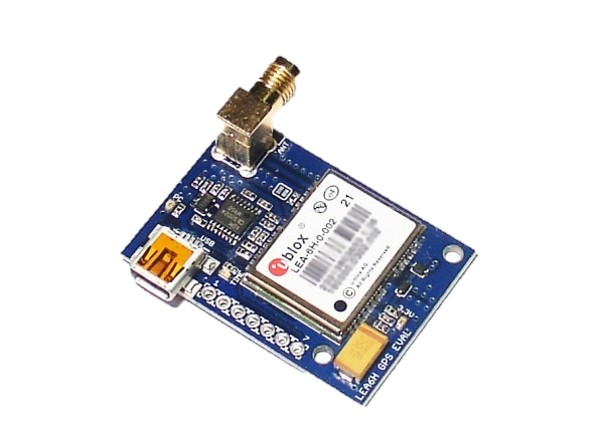
\includegraphics[width=0.5\textwidth]{figures/gpsNoBack.jpg}
  \caption{CGS Shop Board for uBlox LEA-6T} \label{gpsPicture}
\end{figure}

\subsection*{Data Acquisition System Integration}
The sensors were packaged into a main shield for the Arduino. This shield plugs directly into the Arduino, eliminating the need to disconnect and reconnect wiring. Header pins capable of reading commanded PWM signals to servos were also added on the main board. Future work could include stability derivative estimation, and the header pins provide PWM measurement, which can map to servo angles, if it is assumed the servo is not stalled. The servo signal breakout pins also allowed the data to be easily split into sections with and without commanded throttle for drag polar estimation without thrust.

A second board was developed to integrate the air data system with the main sensor board. This pressure board can be located near a wing tip and provides expandability should additional sensors be desired in the future. It also interfaces with the temperature sensor, which is located in the air flow. Finally, all data was saved to a microSD card attached to the main sensor board. Data was saved in binary format for both increased speed and file size reductions. Once on the ground, the data is converted to meaningful values using a custom MATLAB data parser.
\nomenclature{PWM}{Pulse width modulation}
